%!TEX root = ../dokumentation.tex

\chapter{Angular}
\label{ch:angular}

\section{Allgemein}

\subsection{Einführung in das Framework}
Angular ist ein von Google verwaltetes Open Source Framework für die Entwicklung von Single-Page-Applikationen. Die erste Version des Angular-Frameworks hat den Namen AngularJS. Alle nachfolgenden Versionen tragen den Namen Angular, da es wischen der ersten und zweiten Version des Frameworks grundlegende Änderungen gab. Das Framework wird kontinuierlich weiterentwickelt. Monatlich soll eine Minor-Version und alle sechs Monate eine Major-Version erscheinen. Die aktuellste stabilste Version von Angular hat die Versionsnummer 7.1.4. \autocites[vgl.][vii\psqq]{Woiwode.2018}[vgl.][3\psqq]{Freeman.2018}

Das Framework selbst ist in der Sprache TypeScript geschrieben. Angular kann mit TypeScript, JavaScript oder Dart genutzt werden. \autocites[vgl.][vii\psq]{Woiwode.2018}[vgl.][13]{Steyer.2017}

Das in \autoref{} beschriebene MVC Entwurfsmuster kann in einer Angular-Anwendung umgesetzt werden. Die \autoref{ } zeigt die einzelnen Bestandteile der Anwendung. Dabei implementiert das Template die View, die Komponente den Controller und das Modell das Model. \autocite[vgl.][34\psqq]{Freeman.2018} Im weiteren Verlauf werden die Bestandteile näher beschrieben. 

\comment{Abbildung von \textcite[][35]{Freeman.2018}}


\subsection{Vorbereitung der Entwicklungsumgebung}
%% Hier besonders Angular Cli beschreiben
Für die Entwicklung einer Angular-Anwendung wird unter anderem NodeJS, AngularCLI, eine Entwicklungsumgebung und ein Browser benötigt.  

Sowohl \textcite[vgl.][3\psqq]{Woiwode.2018} als auch \textcite[vgl.][3\psqq]{Steyer.2017} empfehlen die Verwendung der frei verfügbaren Entwicklungsumgebung Visual Studio Code. Die Entwicklungsumgebung unterstützt die Entwicklung in TypeScript und lässt sich leicht durch Plug-Ins, die die Entwicklung erleichtern sollen, erweitern. Visual Studio Code ist für Linux, Mac und Windows verfügbar und kann unter \url{https://code.visualstudio.com/Download}  heruntergeladen werden.

Die JavaScript Laufzeitumgebung \textit{NodeJS} ermöglicht das Ausführen von JavaScript Code auf dem Server. Einige Tools, die zur Entwicklung einer Angular-Anwendung verwendet werden, verwenden NodeJS. Außerdem bietet NodeJS einige Pakete mit wiederverwendbarem Code, die über den in integrierten Paketmanager \textit{npm} installiert werden können. Die aktuellste Version kann von \url{https://nodejs.org/} heruntergeladen und installiert werden. 

Das Angular Commandline Interface (kurz: AngularCLI) unterstützt den Entwickler beim Erzeugen und Verwalten einer Angular-Anwendung. AngularCLI erzeugt unter anderem  das Grundgerüst einer Angular-Anwendung und richtet den TypeScript Compiler, Werkzeuge zur Testautomatisierung und den Build-Prozess ein. Die aktuelle Version von AngularCLI kann über den Paketmanager \textit{npm} siehe \autoref{lst:InstallAngularCLI} installiert werden. \autocites[vgl.][1\psqq]{Steyer.2017}[vgl.][7\psqq]{Freeman.2018}[vgl.][6\psqq]{Woiwode.2018} 

%Teilweise ist das von AngularCLI generierte Projekt für den Anwendungsfall nicht ausreichend. Für diesen Fall gibt es weitere Möglichkeiten. \textcite[vgl.][8\psq]{Steyer.2017} beschreibt diese Möglichkeiten in seinem Buch. 

\begin{lstlisting}[caption=Installation von AngularCLI, label=lst:InstallAngularCLI, language=bash]
npm install -g @angular/cli
\end{lstlisting}

Struktur einer durch AngularCLI erzeugte Angular-Anwendung:
\comment{Evtl. an dieser Stelle den Source Code Ordner weg lassen und näher auf die anderen Dateien eingehen.}
\begin{tabbing}
	mm \= mm \= mmmmmmmmmmmmmmmm \= \kill
	$\vdash$ \textbf{example/} \\ 
	| \> $\vdash$ \textbf{src/}\\ 
	| \> \> $\vdash$  \textbf{app/}\\
	| \> \>  --app.component.css  $\Rightarrow$ \textit{CSS-Datei von AppComponent}\\ 
	| \> \>  --app.component.html  $\Rightarrow$ \textit{Template von AppComponent}\\
	| \> \>  --app.component.ts	 $\Rightarrow$ \textit{Komponente AppComponent}\\
	| \> \>  --app.module.ts  $\Rightarrow$ \textit{Root-Modul AppModule}\\
	%| \> \>  --hello.component.ts  $\Rightarrow$ \textit{Komponente HelloComponent}\\
	| \> \> $\vdash$ \textbf{assets/} \\
	| \> \> $\vdash$ \textbf{environments/} \\
	| \> --index.html\\
	| \> --main.ts\\
	| \> --styles.css \\
	| \> --... \\
	| \> $\vdash$ \textbf{node\_modules/}\\ 
	| \> $\vdash$ \textbf{e2e/}\\   
	| --...\\
\end{tabbing}


\section{Grundkonzepte}


\comment{Wie setzt Angular das MVC Pattern um? Abbildung S.35 Freeman - kurze Beschreibung und dann lange Beschreibung durch Unterkapitel} 

Im Folgenden werden die in Angular verwendeten Konzepte näher erläutert. Die Beispielanwendung in \autoref{fig:AngularAnwendung} wird zur Erklärung der Konzepte verwendet. Bei Änderung des Namens im Input-Feld wird dieser in der obigen Überschrift auch verändert.

\begin{figure}
	\centering
	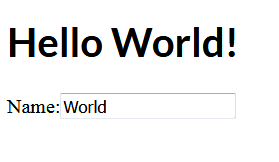
\includegraphics{angular-anwendung.png}
	\caption{Screenshot Angular-Beispielanwendung} 
	\label{fig:AngularAnwendung}
\end{figure}



%% Erklärung am Beispiel des Initialen Projekts --> Mit Hinweis darauf, dass dies Projekt beliebig erweitert werden kann.
\subsection{Angular-Module}

%%Funktion von Modulen
Eine Angular-Anwendung ist modular aufgebaut und kann demnach aus mehreren Angular-Modulen bestehen. Angular-Module sind nicht mit den in \autoref{sec:der-sprachstandard-ecmascript} vorgestellten JavaScript-Modulen zu verwechseln. \autocites[vgl.][103\psqq]{Steyer.2017}[vgl.][301\psqq]{Woiwode.2018} Die Module einer Angular-Anwendung können in Root-Module, Feature-Module und Shared-Module unterteilt werden. 

\comment{Den Begriff Bootstrapping erwähnen!}
%%Bootstrapping
Wenn ein Client eine auf Angular basierte Seite anfordert, dann schickt der Server den Inhalt der \textit{index.html} als Antwort an den Client zurück. Der Client führt daraufhin die im HTML-Dokument enthaltenen Skript-Elemente aus. Dabei wird die Angular-Plattform initialisiert und das Root-Modul übergeben. Dieses Root-Modul konfiguriert die Angular-Anwendung.\autocites[vgl.][60]{Steyer.2017}[vgl.][226\psqq]{Freeman.2018}  Das Root-Modul der Beispielanwendung ist das Modul \textit{AppModule} siehe \autoref{lst:AppModule}. 

%Dekorator und Eigenschaften
Module werden im Allgemeinen durch den Dekorator \textit{@NgModule} gekennzeichnet. Ein Modul kann verschiedene weitere Module über die Eigenschaft \textit{import} importieren und damit die bereitgestellten Funktionalitäten verwenden. Die vom Modul verwendeten Direktiven, Komponenten und Pipes werden in der Eigenschaft \textit{declarations} angegeben. Jedes Root-Modul besitzt die Eigenschaft \textit{bootstrap}. Diese Eigenschaft spezifiziert die Komponente, die beim Starten der Anwendung geladen werden soll. 

%% Beschreibung am Beispiel
Das Modul \textit{AppModule} in \autoref{lst:AppModule} importiert die Module \textit{NgModule}, \textit{BrowserModule} und \textit{FormsModule} und deklariert die zugehörigen Komponenten \textit{AppComponent} und \textit{HelloComponent}. Beim Starten der Anwendung soll die Komponente \textit{AppComponent} aufgerufen werden.

\begin{lstlisting}[caption=Das Root-Module in der Datei app.module.ts, label=lst:AppModule, language=Java]
import { NgModule } from '@angular/core';
import { BrowserModule } from '@angular/platform-browser';
import { FormsModule } from '@angular/forms';

import { AppComponent } from './app.component';
import { HelloComponent } from './hello.component';

@NgModule({
	imports:      [ BrowserModule, FormsModule ],
	declarations: [ AppComponent, HelloComponent ],
	bootstrap:    [ AppComponent]
})
export class AppModule { }

\end{lstlisting}

%%Feature-Module und Shared-Module
Feature Modulen ermöglichen die Gruppierung einer Anwendung in Anwendungsfällen. Mithilfe von Shared-Module können die Teile einer Anwendung zusammengefasst werden, die unabhängig vom Anwendungsfall verwendet werden können. \autocites[vgl.][528\psqq]{Freeman.2018}[vgl.][]{Google.c}[vgl.][105\psqq]{Steyer.2017}

\subsection{Komponenten}

\comment{Evtl. auf den Lifecycle von Komponenten eingehen.}

%%Beschreibung von Komponenten
Komponenten sind Klassen, die Daten und Logik zur Anzeige in den zugehörigen Templates bereitstellen. Diese ermöglichen die Aufteilung einer Angular-Anwendung in logisch getrennte Teile. \autocite[vgl.][401]{Freeman.2018} 

%%Dekorator und Eigenschaften von Komponente
Eine Komponente wird durch den Dekorator \textit{@Component} gekennzeichnet und kann über verschiedene Dekorator-Eigenschaften konfiguriert werden. Die Eigenschaft \textit{selector} identifiziert das HTML-Element, dass durch diese Komponente repräsentiert wird. Zur Anzeige der bereitgestellten Daten kann entweder ein Inline-Template \textit{template} definiert oder auf ein externes Template \textit{templateUrl} verwiesen werden. \autocites[vgl.][]{Google.b}[vgl.][405]{Freeman.2018}[vgl.][47\psqq]{Steyer.2017}

\comment{Beschreibung von Input- und Output Eigenschaften.}

%%Beschreibung des Beispiels
Die Beispielanwendung enthält die Komponenten \textit{AppComponent} (siehe \autoref{lst:AppComponentTs}) und \textit{HelloComponent} (siehe \autoref{lst:HelloComponentTs}).

\begin{lstlisting}[caption=Die Komponente AppComponent in der Datei app.component.ts, label=lst:AppComponentTs, language=Java]
import { Component } from '@angular/core';

@Component({
selector: 'my-app',
	templateUrl: './app.component.html',
	styleUrls: [ './app.component.css' ]
})
export class AppComponent  {
	name: string;
}
\end{lstlisting}

\begin{lstlisting}[caption=Die Komponente HelloComponent in der Datei hello.component.ts, label=lst:HelloComponentTs, language=Java]
import { Component, Input } from '@angular/core';

@Component({
	selector: 'hello',
	template: `<h1>Hello {{name}}!</h1>`,
	styles: [`h1 { font-family: Lato; }`]
})
export class HelloComponent  {
	@Input() name: string;
}
\end{lstlisting}

\subsection{Templates}
%%Beschreibung von Templates
Zur Darstellung von Komponenten nutzt Angular Templates. Ein Template besteht aus HTML Code, der um Angular spezifische Konzepte wie Direktiven, Datenbindungsausdrücke und Pipes erweitert wird. \autocites[vgl.][]{Google.b}[vgl.][52]{Steyer.2017} 

%% Beschreibung der unterschiedlichen Direktiven
Mit Direktiven kann einem Element zusätzliches Verhalten hinzugefügt werden. \autocites[vgl.][265]{Steyer.2017}[vgl.][401]{Freeman.2018} In Angular werden folgende drei Arten von Direktiven unterschieden. \autocite[vgl.][]{Google.}

\begin{itemize}
	\item Strukturelle Direktiven 
	\item Attribut-Direktiven
	\item Komponenten
\end{itemize}

%%Strukturelle Direktive
Die strukturellen Direktiven ändern die Struktur des zugehörigen HTML-Elements, indem sie HTML-Elemente hinzufügen oder entfernen. Hierfür verwenden die strukturellen Direktiven Templates, die beliebig oft gerendert werden. \autocites[vgl.][269\psqq]{Steyer.2017}[vgl.][365]{Freeman.2018} Beispiele für strukturellen Direktiven aus Angular sind \autocite[vgl.][261\psqq]{Freeman.2018}:
\begin{description}
	\item [ngIf] Fügt dem HTML-Dokument Inhalt hinzu, wenn die Bedingung wahr ist. 
	\item [ngfor] Fügt für jedes Item einer Datenquelle den gleichen Inhalt dem HTML-Dokument hinzu.
	\item [ngSwitch] Fügt dem HTML-Dokument, abhängig vom Wert eines Ausdrucks, Inhalt hinzu.
\end{description} 

%%Attribut-Direktive
Das Verhalten und das Aussehen des zugehörigen HTML-Elements kann durch die Attribut-Direktiven verändert werden. Diese Direktiven fügen oder entfernen dem zugehörigen HTML-Element Attribute. \autocite[vgl.][339]{Freeman.2018} Beispiele für Attribut-Direktiven aus Angular-JS \autocite[vgl.][249\psqq]{Freeman.2018}:
\begin{description}
	\item [ngStyle] Mit dieser Direktive können unterschiedliche Style-Eigenschaften dem Element hinzugefügt werden.
	\item [ngClass] Weißt dem Element ein oder mehrere Klassen hinzu. 
\end{description}

%%Komponente Direktive
Mittels einer Komponente kann einem HTML-Element eine View hinzugefügt werden. Komponenten sind nämlich Direktiven mit einer eigenen View. \autocites[vgl.][265]{Steyer.2017}

Die von Angular bereitgestellten Direktiven (engl. Built-In Directives) können durch selbst entwickelte Direktiven erweitert werden. \autocite[vgl.][261]{Freeman.2018}

%%Datenbindungsausdrücke
Der Datenaustausch zwischen der Komponente und dem Template erfolgt durch Datenbindungsausdrücke. Ein Datenbindungsausdruck bindet einen JavaScript-Ausdruck an ein Ziel. Das Ziel kann entweder eine Attribut-Direktive oder eine Eigenschaft des zugehörigen HTML-Elements sein. Der JavaScript-Ausdruck ermöglicht den Zugriff auf die Eigenschaften und Methoden der Komponente. \autocites[vgl.][237\psqq]{Freeman.2018}[vgl.][52\psq]{Steyer.2017} [vgl.][]{Google.d} Es gibt insgesamt drei Arten von Data-Bindings, die anhand der Flussrichtung der Daten unterschieden werden können. 

\begin{table}
\begin{tabular}{|>{\raggedright\arraybackslash}p{3cm}|>{\raggedright\arraybackslash}p{3.2cm}|>{\raggedright\arraybackslash}p{6.5cm}|}
	\hline
	\textbf{Richtung}&\textbf{Syntax}&\textbf{Verwendung}\\
	\hline 
	One-way Komponente -> View &\{\{Ausdruck\}\} \lbrack Ziel\rbrack =\dq Ausdruck\dq  & Interpolation, Eigenschaft, Attribut, Klasse, Style\\ 
	\hline 
	One-way Komponente <- View &(Ziel)=\dq Ausdruck\dq&Events\\ 
	\hline 
	Two-way&\lbrack (Ziel)\rbrack =\dq Ausdruck\dq&Formular\\ 
	\hline 
\end{tabular}
\caption{Arten von Data-Bindings}
\label{tab:DataBinding}
\end{table}

%%Pipes
Mit Pipes können die  Daten vor der Ausgabe sortiert, formatiert oder gefiltert werden. \autocite[vgl.][83\psqq]{Steyer.2017}

\begin{lstlisting}[caption=Das Template in der Datei app.component.html, label=lst:AppComponentHTML, language=HTML]
<hello name="{{name}}"></hello>
<label for="name">Name:</label>
<input name="name" [(ngModel)]="name">
\end{lstlisting}

\subsection{Services}
Laut \textcite[vgl.][474]{Freeman.2018} kann jedes Objekt, dass durch Dependency Injection verwaltet und verteilt wird, als Service bezeichnet werden. Services stellen wiederverwendbare Routinen oder Daten zur Verfügung, die von Direktiven, Komponenten, weiteren Services und Pipes verwendeten werden können. \autocites[vgl.][467\psqq]{Freeman.2018}[vgl.][89]{Steyer.2017}

Services verringern die Abhängigkeiten zwischen den Klassen, durch Dependency Injection. Hierdurch können Beispiel Unit-Tests einfacher durchgeführt werden. \autocite[vgl.][469]{Freeman.2018} 

%%Wie kann ein Service verwendet werden? 
%%Registrierung
Um einen Service zu verwenden, muss dieser entweder global in einem Modul oder lokal in einer Komponente registriert werden. Dies geschieht durch Einrichten eines Providers beim Modul oder der Komponente. Der Provider verknüpft ein Token mit einem Service. Ein Service kann eine Klasse, ein Wert, eine Funktion, eine Factory oder eine Weiterleitung sein. Aus diesem Grund gibt es unterschiedliche Provider.

%%Ergebnis der Registrierung
Sobald ein Service global registrierte wurde, steht dieser auch in weiteren Modulen zur Verfügung. Ein lokal registrierter Service kann dahingegen nur von der jeweiligen Komponente und den direkten und indirekten Kindkomponenten verwendet werden. 

%%Nutzung
Zur Nutzung eines Services muss die jeweilige Klasse den Service importieren und im Konstruktor deklarieren. Beim Erzeugen einer Instanz der Klasse injiziert Angular den jeweiligen Service.\autocites[vgl.][92\psqq]{Steyer.2017}[vgl.][474\psqq]{Freeman.2018}

\comment{Evtl. noch einen kurzen Abschnitt zu Routen}

\section{Verwendung}    